% answers.tex —— 1977 年·河南卷 · 参考答案与详细解析片段
% 由 tools/generate_projects.py 依来源总账自 1977/1977_数学真题_河南_试题.md + 1977/1977_数学真题_河南_解析正文.md + 1977/1977_数学真题_河南_答案要点.md 生成，勿手改（改源 MD 后重跑）


\begin{gktip}
固定源是题面与解答连续出现的扫描材料。下文逐题对照源解答并重新计算关键结论；第 8 题保留源卷对二次项系数的更正，第 9 题源卷的（1）、（3）跳号已按本库小问连续编号规范重排为（1）、（2）。
\end{gktip}

\begin{answer}
\gksolhead{1}{}

\textbf{题目}（7 分）：

\Needspace{5\baselineskip}
化简下式：

\nopagebreak[4]
\[
(1-c^2)^{-\frac12}
-\left\{[(1+c)(1-c)]^{\frac12}
+c^2[(1+c)(1-c)]^{-\frac12}\right\}.
\]

\Needspace{4\baselineskip}
\textbf{解析}

\Needspace{5\baselineskip}
令 $u=1-c^2=(1+c)(1-c)$。在原式有意义的条件下，

\nopagebreak[4]
\[
\begin{aligned}
&(1-c^2)^{-\frac12}
-\left\{[(1+c)(1-c)]^{\frac12}
+c^2[(1+c)(1-c)]^{-\frac12}\right\}\\
&=u^{-\frac12}-u^{\frac12}-c^2u^{-\frac12}\\
&=u^{-\frac12}\bigl[1-u-c^2\bigr]\\
&=u^{-\frac12}\bigl[1-(1-c^2)-c^2\bigr]=0.
\end{aligned}
\]

\gkanswer{答案：$0$。}

\end{answer}
\begin{answer}
\gksolhead{2}{}

\textbf{题目}（7 分）：

\Needspace{5\baselineskip}
求

\nopagebreak[4]
\[
\frac{\lg3+\lg2}
{\frac14\lg16+\sqrt{(\lg1-\lg10)^2}+\frac12\lg0.09}
\]

的值。

\Needspace{4\baselineskip}
\textbf{解析}

利用 $\lg16=4\lg2$、$\lg1=0$、$\lg10=1$ 以及
\Needspace{5\baselineskip}
$\frac12\lg0.09=\lg0.3=\lg3-\lg10$，原式为

\nopagebreak[4]
\[
\frac{\lg3+\lg2}
{\lg2+\sqrt{(0-1)^2}+\lg0.3}
=\frac{\lg3+\lg2}{\lg2+1+\lg3-1}=1.
\]

\gkanswer{答案：$1$。}

\end{answer}
\begin{answer}
\gksolhead{3}{}

\textbf{题目}（7 分）：

\Needspace{5\baselineskip}
求等式

\nopagebreak[4]
\[
5^{x^2-2x}=125
\]

中 $x$ 的值。

\Needspace{4\baselineskip}
\textbf{解析}

\Needspace{5\baselineskip}
因为 $125=5^3$，所以

\nopagebreak[4]
\[
5^{x^2-2x}=5^3
\quad\Longrightarrow\quad
x^2-2x=3.
\]

\Needspace{5\baselineskip}
于是

\nopagebreak[4]
\[
(x-3)(x+1)=0,
\qquad x=3\ \text{\text{或}}\ x=-1.
\]

\gkanswer{答案：$x=3$ 或 $x=-1$。}

\end{answer}
\begin{answer}
\gksolhead{4}{}

\textbf{题目}：

\Needspace{5\baselineskip}
已知 $a\text{、}b\text{、}c$ 分别表示 $\triangle ABC$ 的角 $A\text{、}B\text{、}C$ 对边的长，求证：

\nopagebreak[4]
\[
a(\sin B-\sin C)+b(\sin C-\sin A)+c(\sin A-\sin B)=0.
\]

\Needspace{4\baselineskip}
\textbf{解析}

\Needspace{5\baselineskip}
由正弦定理，

\nopagebreak[4]
\[
\frac a{\sin A}=\frac b{\sin B}=\frac c{\sin C}.
\]

\Needspace{5\baselineskip}
因此

\nopagebreak[4]
\[
a\sin B=b\sin A,\qquad
a\sin C=c\sin A,\qquad
b\sin C=c\sin B.
\]

\Needspace{5\baselineskip}
将左端展开并按这些等式替换：

\nopagebreak[4]
\[
\begin{aligned}
& a(\sin B-\sin C)+b(\sin C-\sin A)+c(\sin A-\sin B)\\
&=a\sin B-a\sin C+b\sin C-b\sin A+c\sin A-c\sin B\\
&=b\sin A-c\sin A+c\sin B-b\sin A+c\sin A-c\sin B\\
&=0.
\end{aligned}
\]

\gkanswer{答案：见解析版}

\end{answer}
\begin{answer}
\gksolhead{5}{}

\textbf{题目}（8 分）：

如图，已知正方形 $ABCD$ 的边 $CD$ 上任意一点 $E$，延长 $BC$ 到 $F$，使 $CF=CE$，设 $BE$ 与 $DF$ 相交于 $G$，求证 $BG\perp DF$。

\begin{gktip}
原源 PDF 第 2 页附有正方形、延长线和交点 $G$ 的示意图；LaTeX 版按源图重绘。
\end{gktip}
\nopagebreak[4]
\begin{center}% 1977 年河南卷第五题：正方形 ABCD（A 左上、D 右上、B 左下、C 右下），
% E 在 DC 边上，F 在 BC 延长线上（CF=CE），BE 与 DF 交于 G（按源卷第 2 页布局）
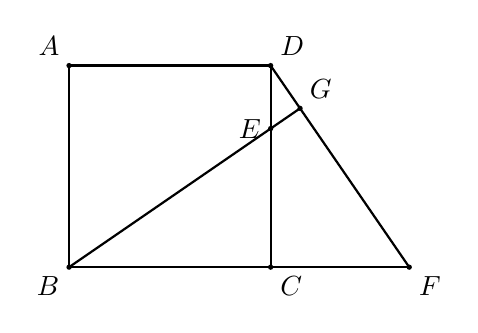
\begin{tikzpicture}[scale=0.8]
  \coordinate (A) at (0,3.2);
  \coordinate (D) at (3.2,3.2);
  \coordinate (C) at (3.2,0);
  \coordinate (B) at (0,0);
  \coordinate (E) at (3.2,2.2);
  \coordinate (F) at (5.4,0);
  \coordinate (G) at (3.667,2.521);
  \draw[thick] (A)--(D)--(C)--(B)--cycle;
  \draw[thick] (C)--(F);
  \draw[thick] (B)--(G);
  \draw[thick] (D)--(F);
  \fill (A) circle (1.2pt) node[above left] {$A$};
  \fill (D) circle (1.2pt) node[above right] {$D$};
  \fill (C) circle (1.2pt) node[below right] {$C$};
  \fill (B) circle (1.2pt) node[below left] {$B$};
  \fill (E) circle (1.2pt) node[left] {$E$};
  \fill (F) circle (1.2pt) node[below right] {$F$};
  \fill (G) circle (1.2pt) node[above right] {$G$};
\end{tikzpicture}
\end{center}
\nopagebreak[4]
\Needspace{4\baselineskip}
\textbf{解析}

在直角三角形 $\triangle BCE$ 和 $\triangle DCF$ 中，
\Needspace{5\baselineskip}
$BC=CD$（正方形的边相等），$CE=CF$（已知），且两者均在 $C$ 点为直角。因此

\nopagebreak[4]
\[
\triangle BCE\cong\triangle DCF.
\]

\Needspace{5\baselineskip}
从而

\nopagebreak[4]
\[
\angle GBC=\angle FDC.
\]

\Needspace{5\baselineskip}
又因为

\nopagebreak[4]
\[
\angle EBC+\angle BEC=90^\circ,
\qquad
\angle BEC=\angle DEG
\]

\Needspace{5\baselineskip}
（对顶角相等），所以

\nopagebreak[4]
\[
\angle FDC+\angle DEG=90^\circ.
\]

\Needspace{5\baselineskip}
其中 $DG$ 在 $DF$ 上、$BG$ 在 $BE$ 上，故 $\angle DGB=90^\circ$，即

\nopagebreak[4]
\[
BG\perp DF.
\]

\gkanswer{答案：$BG\perp DF$。}

\end{answer}
\begin{answer}
\gksolhead{6}{}

\textbf{题目}（10 分）：

\Needspace{5\baselineskip}
求证：

\nopagebreak[4]
\[
\operatorname{tg}^2\alpha-\operatorname{ctg}^2\alpha
=-\frac{2\sin4\alpha}{\sin^3 2\alpha}.
\]

\Needspace{4\baselineskip}
\textbf{解析}

\Needspace{5\baselineskip}
在 $\sin\alpha\cos\alpha\ne0$ 且 $\sin2\alpha\ne0$ 的定义条件下，

\nopagebreak[4]
\[
\begin{aligned}
\tan^2\alpha-\cot^2\alpha
&=\frac{\sin^4\alpha-\cos^4\alpha}
{\sin^2\alpha\cos^2\alpha}\\
&=\frac{\sin^2\alpha-\cos^2\alpha}
{\frac14\sin^22\alpha}\\
&=-\frac{4\cos2\alpha}{\sin^22\alpha}\\
&=-\frac{2\sin4\alpha}{\sin^32\alpha}.
\end{aligned}
\]

\gkanswer{答案：见解析版}

\end{answer}
\begin{answer}
\gksolhead{7}{}

\textbf{题目}（10 分）：

已知长方体的对角线长为 $L$，它与底面所成的角为 $\alpha$，底面两条对角线的夹角为 $\beta$，求长方体的体积。

\begin{gktip}
原源 PDF 第 3 页附有长方体和底面对角线夹角示意图；LaTeX 版按源图重绘。
\end{gktip}
\nopagebreak[4]
\begin{center}% 1977 年河南卷第七题：长方体 ABCD-A1B1C1D1（顶面 A1B1C1D1），
% 体对角线 A1C（虚线）与底面所成角 α 标在 C 处，底面对角线 AC、BD 夹角 β 标在中心（按源卷第 3 页布局）
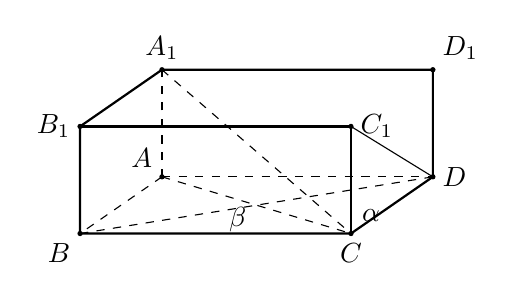
\begin{tikzpicture}[scale=0.8]
  \coordinate (B) at (0,0.8);
  \coordinate (C) at (4.3,0.8);
  \coordinate (D) at (5.6,1.7);
  \coordinate (A) at (1.3,1.7);
  \coordinate (B1) at (0,2.5);
  \coordinate (C1) at (4.3,2.5);
  \coordinate (D1) at (5.6,3.4);
  \coordinate (A1) at (1.3,3.4);
  \draw[thick] (B)--(C)--(D)--(D1)--(A1)--(B1)--cycle;
  \draw[thick] (B)--(B1);
  \draw[thick] (C)--(C1);
  \draw[thick] (A1)--(D1);
  \draw[thick] (B1)--(C1);
  \draw[thin] (C1)--(D);
  \draw[dashed] (A)--(B);
  \draw[dashed] (A)--(D);
  \draw[dashed] (A)--(A1);
  \draw[dashed] (A)--(C);
  \draw[dashed] (B)--(D);
  \draw[dashed] (A1)--(C);
  \fill (A) circle (1.2pt) node[above left] {$A$};
  \fill (B) circle (1.2pt) node[below left] {$B$};
  \fill (C) circle (1.2pt) node[below] {$C$};
  \fill (D) circle (1.2pt) node[right] {$D$};
  \fill (A1) circle (1.2pt) node[above] {$A_1$};
  \fill (B1) circle (1.2pt) node[left] {$B_1$};
  \fill (C1) circle (1.2pt) node[right] {$C_1$};
  \fill (D1) circle (1.2pt) node[above right] {$D_1$};
  \node at (4.62,1.08) {$\alpha$};
  \node at (2.5,1.02) {$\beta$};
\end{tikzpicture}
\end{center}
\nopagebreak[4]
\Needspace{4\baselineskip}
\textbf{解析}

\Needspace{5\baselineskip}
设长方体的高为 $h$，底面一条对角线为 $d$。由对角线与底面所成的角，

\nopagebreak[4]
\[
h=L\sin\alpha,\qquad d=L\cos\alpha.
\]

\Needspace{5\baselineskip}
底面矩形的两条对角线长度相等，夹角为 $\beta$，故底面积

\nopagebreak[4]
\[
S=\frac12d^2\sin\beta
=\frac12L^2\cos^2\alpha\sin\beta.
\]

\Needspace{5\baselineskip}
所以体积

\nopagebreak[4]
\[
V=hS
=\frac12L^3\cos^2\alpha\sin\alpha\sin\beta.
\]

\gkanswer{答案：$V=\dfrac12L^3\cos^2\alpha\sin\alpha\sin\beta$。}

\end{answer}
\begin{answer}
\gksolhead{8}{}

\textbf{题目}（14 分）：

\Needspace{5\baselineskip}
某工厂科研小组，对一项生产工艺过程总结出产量指标函数和消耗函数为：

\nopagebreak[4]
\[
f_1(x)=a_1x^2+\frac12x+c
\qquad\text{\text{和}}\qquad
f_2(x)=a_2x^2+bx+\frac54\quad\text{（※）}
\]

\Needspace{5\baselineskip}
且知

\nopagebreak[4]
\[
f_1(-1)=f_2(-1)=f_1(3)=f_2(3)=2.
\]

（1） 分别求出产量指标函数 $f_1(x)$ 和消耗函数 $f_2(x)$ 的具体表达式；

（2） 问因素 $x$ 取何值时，$f_1(x)$ 和 $f_2(x)$ 有最大值或最小值？最大值或最小值各是多少？

（3） 画出所求出函数的略图。

\begin{gktip}
\textbf{源注}：原题中 $a_1=a_2=a$，问题无解；源解答注明“酌情把 $f_1(x)$ 和 $f_2(x)$ 中的二次项系数分别改为 $a_1$ 和 $a_2$”。本文按该源注所对应的可解题面转录，并保留这一更正说明。
\end{gktip}

\Needspace{4\baselineskip}
\textbf{解析}

\gksubpart{（1）}

\Needspace{5\baselineskip}
由 $f_1(-1)=f_1(3)=2$ 得

\nopagebreak[4]
\[
\begin{cases}
a_1-\frac12+c=2,\\
9a_1+\frac32+c=2,
\end{cases}
\qquad
a_1=-\frac14,\quad c=\frac{11}{4}.
\]

\Needspace{5\baselineskip}
由 $f_2(-1)=f_2(3)=2$ 得

\nopagebreak[4]
\[
\begin{cases}
a_2-b+\frac54=2,\\
9a_2+3b+\frac54=2,
\end{cases}
\qquad
a_2=\frac14,\quad b=-\frac12.
\]

\Needspace{5\baselineskip}
因此

\nopagebreak[4]
\[
f_1(x)=-\frac14x^2+\frac12x+\frac{11}{4}
=-\frac14(x-1)^2+3,
\]

\nopagebreak[4]
\[
f_2(x)=\frac14x^2-\frac12x+\frac54
=\frac14(x-1)^2+1.
\]

\gksubpart{（2）}

所以 $f_1(x)$ 在 $x=1$ 取极大值 $3$，$f_2(x)$ 在 $x=1$ 取极小值 $1$。

\gksubpart{（3）}

两函数均经过 $(-1,2)$、$(3,2)$；略图按这两个交点与两顶点 $(1,3)$、$(1,1)$ 的位置绘制：
\nopagebreak[4]
\begin{center}% 1977 年河南卷第八题(3)：f1(x)=-1/4(x-1)^2+3（开口向下，实线）
% 与 f2(x)=1/4(x-1)^2+1（开口向上，虚线）的略图（按源卷第 4 页布局：x 轴 -1..4，y 轴刻度 1、2、3）
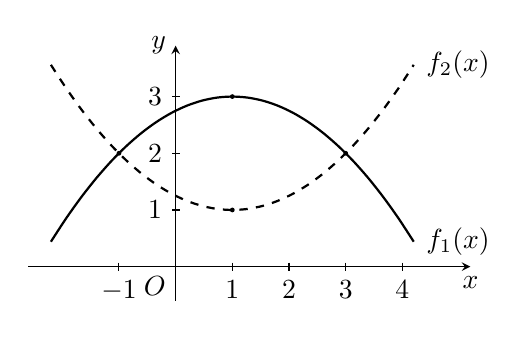
\begin{tikzpicture}[scale=0.72,>=stealth]
  \draw[->] (-2.6,0)--(5.2,0) node[below] {$x$};
  \draw[->] (0,-0.6)--(0,3.9) node[left] {$y$};
  \node[below left] at (0,0) {$O$};
  \foreach \x in {-1,1,2,3,4}{
    \draw[thin] (\x,0.07)--(\x,-0.07) node[below] {$\x$};
  }
  \foreach \y in {1,2,3}{
    \draw[thin] (0.07,\y)--(-0.07,\y) node[left] {$\y$};
  }
  \draw[thick,domain=-2.2:4.2,smooth] plot (\x,{-0.25*(\x-1)*(\x-1)+3});
  \draw[thick,dashed,domain=-2.2:4.2,smooth] plot (\x,{0.25*(\x-1)*(\x-1)+1});
  \fill (1,3) circle (1.2pt);
  \fill (1,1) circle (1.2pt);
  \fill (-1,2) circle (1.2pt);
  \fill (3,2) circle (1.2pt);
  \node[right] at (4.25,0.44) {$f_1(x)$};
  \node[right] at (4.25,3.56) {$f_2(x)$};
\end{tikzpicture}
\end{center}
\nopagebreak[4]
\begin{gktip}
\textbf{源注复核}：若强行令 $a_1=a_2=a$，上述两个方程组的二次项系数互相矛盾，原题无解。固定源明确说明将两函数的二次项系数分别记为 $a_1\text{、}a_2$，本文按该说明整理。
\end{gktip}

\gkanswer{答案（1）：$f_1(x)=-\dfrac14x^2+\dfrac12x+\dfrac{11}{4}=-\dfrac14(x-1)^2+3$；$f_2(x)=\dfrac14x^2-\dfrac12x+\dfrac54=\dfrac14(x-1)^2+1$。}

\gkanswer{答案（2）：$f_1(x)$ 在 $x=1$ 处取极大值 $3$；$f_2(x)$ 在 $x=1$ 处取极小值 $1$。}

\gkanswer{答案（3）：见解析版}

\end{answer}
\begin{answer}
\gksolhead{9}{}

\textbf{题目}（14 分）：

已知过点 $P(0,3\sqrt2)$ 且斜率为 $k$ 的直线与圆心在原点、半径为 $3$ 的圆相交于 $M\text{、}N$ 两点。

（1） 求 $M\text{、}N$ 的坐标；

（2） 问当 $M\text{、}N$ 两点重合时，$k$ 为何值？过 $P$ 点的直线与圆的位置关系如何？这样的直线有几条？它们的夹角是多大？

\begin{gktip}
\textbf{题号说明}：固定源第 4—5 页在第九题中直接印作“（1）”和“（3）”，未见“（2）”题干。本库题库规范要求小问连续编号，故将源卷“（3）”重排为“（2）”，未增删任何题干内容。
\end{gktip}

\Needspace{4\baselineskip}
\textbf{解析}

\gksubpart{（1）}

\Needspace{5\baselineskip}
直线方程为

\nopagebreak[4]
\[
y-3\sqrt2=kx,
\]

\Needspace{5\baselineskip}
圆方程为

\nopagebreak[4]
\[
x^2+y^2=9.
\]

\Needspace{5\baselineskip}
将 $y=3\sqrt2+kx$ 代入圆方程，得

\nopagebreak[4]
\[
(1+k^2)x^2+6\sqrt2\,kx+9=0.
\]

\Needspace{5\baselineskip}
相交的条件是判别式非负，即 $k^2-1\ge0$。两根对应的横坐标为

\nopagebreak[4]
\[
x=\frac{-3\sqrt2\,k\pm3\sqrt{k^2-1}}{1+k^2}.
\]

\Needspace{5\baselineskip}
由 $y=3\sqrt2+kx$，对应纵坐标为

\nopagebreak[4]
\[
y=\frac{3\sqrt2\pm3k\sqrt{k^2-1}}{1+k^2}.
\]

\Needspace{5\baselineskip}
故

\nopagebreak[4]
\[
\begin{aligned}
M&=\left(
\frac{-3\sqrt2\,k+3\sqrt{k^2-1}}{1+k^2},
\frac{3\sqrt2+3k\sqrt{k^2-1}}{1+k^2}
\right),\\
N&=\left(
\frac{-3\sqrt2\,k-3\sqrt{k^2-1}}{1+k^2},
\frac{3\sqrt2-3k\sqrt{k^2-1}}{1+k^2}
\right).
\end{aligned}
\]

\gksubpart{（2）}

\Needspace{5\baselineskip}
当两交点重合时，判别式为零，所以 $k=\pm1$。相应的两条直线为

\nopagebreak[4]
\[
y=x+3\sqrt2,\qquad y=-x+3\sqrt2.
\]

它们与圆相切，且斜率互为负倒数，因此两条切线互相垂直，夹角为 $90^\circ$。

\begin{gktip}
\textbf{源题号说明}：源 PDF 将重合情形印为“（3）”，未见“（2）”；本库规范要求小问连续编号，故重排为“（2）”，未增删题干。
\end{gktip}

\gkanswer{答案（1）：$\begin{aligned}M&=\left(\dfrac{-3\sqrt2\,k+3\sqrt{k^2-1}}{1+k^2},\ \dfrac{3\sqrt2+3k\sqrt{k^2-1}}{1+k^2}\right),\\ N&=\left(\dfrac{-3\sqrt2\,k-3\sqrt{k^2-1}}{1+k^2},\ \dfrac{3\sqrt2-3k\sqrt{k^2-1}}{1+k^2}\right).\end{aligned}$}

\gkanswer{答案（2）：当 $M\text{、}N$ 重合时 $k=\pm1$；此时直线与圆相切，这样的直线有两条：$y=x+3\sqrt2$ 与 $y=-x+3\sqrt2$，其夹角为 $90^\circ$。}

\end{answer}
\begin{answer}
\gksolhead{10}{}

\textbf{题目}：

某电管所为实现农业现代化，加强电力网的建设，沿着一条通往农村的新公路栽电杆。已知一辆汽车每次从电管所运 3 根电线杆，相邻两根电线杆相距 50 米，汽车往返的总路程是 35.5 公里，最后一根电线杆与电管所相距 2450 米。

（1） 第一根电线杆与电管所相距多少？

（2） 共栽了多少根电线杆？

\Needspace{5\baselineskip}
\textbf{参考题 1．（20 分）} 已知

\nopagebreak[4]
\[
x+x^{-1}=2\cos\theta,
\]

\Needspace{5\baselineskip}
求证

\nopagebreak[4]
\[
x^n+x^{-n}=2\cos n\theta.
\]

\textbf{参考题 2．}

\Needspace{5\baselineskip}
（1） 设

\nopagebreak[4]
\[
y=\operatorname{Ln}\left(x+\sqrt{x^2-a^2}\right),
\]

求 $y$ 的导数 $y'$。

\Needspace{5\baselineskip}
（2） 求

\nopagebreak[4]
\[
\int_0^{2p}\sqrt{2px}\,dx
\]

的值。

\Needspace{4\baselineskip}
\textbf{解析}

\gksubpart{（1）}

\Needspace{5\baselineskip}
设第一根电线杆离电管所为 $x$ 米，共栽 $n$ 根。最后一根的位置给出

\nopagebreak[4]
\[
2450=x+(n-1)50.
\]

\Needspace{5\baselineskip}
汽车每次运 3 根，因此共往返 $n/3$ 趟。第一趟往返路程为 $2(x+100)$，最后一趟往返路程为 $2\times2450$，各趟相邻路程相差 $300$ 米。由总路程 $35.5$ 公里，即 $35500$ 米，

\nopagebreak[4]
\[
35500=\frac n3\cdot
\frac{2(x+100)+2\times2450}{2}.
\]

\Needspace{5\baselineskip}
联立得

\nopagebreak[4]
\[
(x,n)=(1000,30)
\quad\text{\text{或}}\quad
(-1050,71).
\]

后一组不符合题意，故第一根电线杆距电管所 $1000$ 米。

\begin{gktip}
\textbf{源注}：源解答中该方程左端印作“$3500$”，系漏零排印——按题面“总行程 $35.5$ 公里”应为 $35500$ 米，且源解答所求得的 $(x,n)=(1000,30)$ 与答句均按 $35500$ 成立。本文按 $35500$ 计算。
\end{gktip}

\gksubpart{（2）}

共栽 $30$ 根。

\textbf{参考题 1}

\Needspace{5\baselineskip}
由

\nopagebreak[4]
\[
x+x^{-1}=2\cos\theta
\]

\Needspace{5\baselineskip}
得

\nopagebreak[4]
\[
x^2-2\cos\theta\,x+1=0,
\qquad
x=\cos\theta\pm i\sin\theta.
\]

\Needspace{5\baselineskip}
于是由棣莫弗公式，

\nopagebreak[4]
\[
\begin{aligned}
x^n+x^{-n}
&=(\cos\theta\pm i\sin\theta)^n
+(\cos\theta\pm i\sin\theta)^{-n}\\
&=\cos n\theta\pm i\sin n\theta
+\cos(-n\theta)\pm i\sin(-n\theta)\\
&=2\cos n\theta.
\end{aligned}
\]

\textbf{参考题 2}

\gksubpart{（1）}

\Needspace{5\baselineskip}
设

\nopagebreak[4]
\[
y=\ln\left(x+\sqrt{x^2-a^2}\right).
\]

\Needspace{5\baselineskip}
则

\nopagebreak[4]
\[
\begin{aligned}
y'
&=\frac{1+\dfrac{x}{\sqrt{x^2-a^2}}}
{x+\sqrt{x^2-a^2}}\\
&=\frac1{\sqrt{x^2-a^2}}.
\end{aligned}
\]

\gksubpart{（2）}

\Needspace{5\baselineskip}
令 $u=2px$，则 $du=2p\,dx$，从而

\nopagebreak[4]
\[
\begin{aligned}
\int_0^{2p}\sqrt{2px}\,dx
&=\frac1{2p}\int_0^{2p}\sqrt{u}\,du\\
&=\frac1{3p}(2p)^{3/2}\bigg|_0^{2p}\\
&=\frac83p^2.
\end{aligned}
\]

\gkanswer{答案（1）：第一根电线杆距电管所 $1000$ 米。}

\gkanswer{答案（2）：共栽 $30$ 根。}

\end{answer}